\documentclass[11pt]{article}
\usepackage[margin=1in]{geometry}
\usepackage{graphicx,booktabs,amsmath,amssymb,microtype,xcolor}
\usepackage{multirow}
\usepackage{caption}
\usepackage[hidelinks]{hyperref}
\usepackage[numbers,sort&compress]{natbib}
\usepackage{algorithm}
\usepackage[noend]{algpseudocode}
\usepackage{placeins}
\usepackage{authblk}
\renewcommand\Authfont{\normalsize}
\renewcommand\Affilfont{\small}
\captionsetup{font=small,labelfont=bf}
\graphicspath{{figures/}}

\newcommand{\ours}{\textsc{EnumRank}}

\title{\bfseries Validity Is Not Recovery:\\Constrained Candidate Selection\\for Molecular String Repair}

\author[1]{Sridhara Syam Chandrabhotla\thanks{All authors contributed equally.
Corresponding author: \texttt{11sridharasyam@gmail.com}}}
\author[2]{KPK Lalitha Vitala}
\author[3]{S.\ Diwakar Bhagavathula}
\affil[1]{Independent Researcher, Bhimavaram, India}
\affil[2]{Department of Electronics and Communications, Vishnu Institute of
Technology, Bhimavaram, India. \texttt{lalitha.v@vishnu.edu.in}}
\affil[3]{Department of Chemistry, SRKR Engineering College, Bhimavaram, India.
\texttt{diwakar.b@srkrec.edu.in}}
\date{}

\begin{document}
\maketitle
\vspace{-2.5em}

\begin{abstract}
\noindent
Generative models for molecules routinely emit SMILES strings that no chemistry
toolkit will parse, and a growing body of work aims to \emph{correct} them.
\emph{Validity}, the fraction of repaired strings that parse, is the headline by
which that work is claimed, even where identity metrics are reported too. We show
validity is a weak proxy for whether the \emph{intended} molecule is recovered,
and that validity-only evaluation can substantially mis-rank recovery systems.

We build a leakage-controlled benchmark of 6{,}000 corrupted SMILES with known
ground truth, drawn from a held-out molecule pool and corrupted with an operator
mix calibrated to the error distribution of real generative-model failures. On
it, a recent published corrector attains 86.6\% validity but recovers the
intended molecule for 1.2\% of inputs: roughly 74 valid molecules per correct
one. An unconstrained large-language-model repair loop shows
the opposite profile (47.7\% validity, 13.8\% recovery), so the two systems are
ordered one way by validity and the other by recovery.

We then show that invalid-SMILES recovery is better formulated as constrained
candidate \emph{selection} than as unconstrained sequence generation. A symbolic
enumerator over single-token edits yields a candidate set containing the ground
truth for 99.79\% of items (median 50 candidates); the toolkit's diagnosis
prunes it losslessly; and a character-level chemical language model ranks what
remains.
The resulting system reaches \textbf{100.0\% validity and 80.7\% exact
recovery}, versus 59.4\% for a supervised sequence-to-sequence corrector trained
on 245{,}000 in-distribution repair pairs, which our method needs none of.
The ranker is trained only on a disjoint molecule split, so the result is not
pretraining contamination. The approach transfers to real
generative-model output: 91.5\% of 4{,}009 genuinely invalid strings sampled
from a character-level generator admit a one-edit repair, and on corruptions of
that generator's own molecules recovery is 78.9\%. On an external benchmark built
with another group's corruption code and molecule corpus, recovery among
reachable items is 87.5\%, and its output is always valid where it answers.
Coverage collapses from 99.7\% to 0.5\% once two errors coincide, bounding the
scope. Ranking confidence supports calibrated abstention: 46\% of all inputs can
be answered at 96.4\% precision.
We release the benchmark, code, and per-item outputs.
\end{abstract}

\vspace{0.5em}
\noindent\textbf{Keywords:} SMILES; molecular string repair; generative models
for molecules; evaluation methodology; chemical language models; benchmark;
neuro-symbolic methods; selective prediction

\section{Background}

Molecular generative models emit molecules as strings, most often
SMILES~\citep{weininger1988smiles}. A well-known failure mode is that a
syntactically plausible string need not denote a molecule: ring-closure digits
may be unbalanced, branches unclosed, valences violated, or an aromatic system
un-kekulizable. Depending on architecture, between a few percent and a large
minority of sampled strings fail to
parse~\citep{brown2019guacamol,polykovskiy2020moses}. Sampling temperature
compounds this: the character-level generator we use throughout falls from
93.3\% valid at $T{=}1.0$ to 85.3\% at $T{=}1.2$ and 64.1\% at $T{=}1.5$.

The dominant response has been prevention: constrained
grammars~\citep{kusner2017grammar,dai2018syntax}, or alternative string
encodings such as SELFIES~\citep{krenn2020selfies}, whose grammar makes every
string decodable. A second and more recent response is correction: take the
broken string and repair it. Correction is attractive because invalid strings are
concentrated where the model is least certain, so discarding them throws away the
model's hardest cases. The premise deserves care, however:
\citet{skinnider2024invalid} shows that the ability to emit invalid strings is
itself beneficial, acting as a self-corrective filter on low-likelihood samples,
and that \emph{enforcing} validity introduces structural bias. That argument
tells against prevention rather than against correction, since a repaired string
is recovered after the fact rather than forced during sampling. It does mean the
case for repair rests on recovering the intended molecule, not merely on raising
a validity count.

Validity is easy to compute, needs no ground truth, and is the number these
systems are named and compared by. It is not the only number reported.
\citet{schoenmaker2023uncorrupt} measure a molecule reconstruction rate of 78\%
and observe that ``fixed molecules do not necessarily represent the original
molecule''; \citet{smiself2025} report exact match to the ground truth alongside
validity; and \citet{amrec} argue the distinction directly. The gap between
validity and identity is therefore known. What has not been established is how
much it costs: whether validity is a mildly noisy proxy for recovery or a
qualitatively different quantity that can order systems the wrong way round.
This paper answers that question, and supplies the benchmark and metrics needed
to ask it of any future system.

\paragraph{The problem with validity.}
Consider a generative model that intended some molecule $m$ and emitted a
corrupted string $\tilde{s}$. A corrector maps $\tilde{s}$ to some string
$\hat{s}$. Validity asks only whether $\hat{s}$ parses. It is fully satisfied by
a corrector that discards $\tilde{s}$ and returns benzene. Nothing in the metric
rewards returning $m$. The concern is not hypothetical: methods that convert a
broken string into a guaranteed-decodable representation achieve near-perfect
validity precisely because the conversion is free to change the molecule.

What a practitioner wants is \emph{recovery}: that $\hat{s}$ denotes $m$. This
is measurable whenever ground truth is available, and it is the quantity we
argue the field should report.

\paragraph{Contributions.}
\begin{enumerate}\itemsep2pt
\item A leakage-controlled recovery benchmark with known ground truth, built
      from a held-out molecule pool and calibrated to the empirical error mix of
      a real generative model (Section~\ref{sec:bench}).
\item A \emph{quantitative} account of how far validity and recovery come
      apart, far enough to reverse the ordering of published systems. That
      validity is insufficient has been argued qualitatively~\citep{amrec};
      we measure the consequence (Section~\ref{sec:exp1}).
\item A transfer of the bounded-edit constrained-selection formulation from
      syntax repair~\citep{considine2025syntax} to molecular strings, instantiated
      with a chemistry toolkit's diagnosis as the pruning constraint and a chemical
      language model as the prior: a six-stage system, \ours{}, attaining 100.0\%
      validity and 80.7\% exact recovery
      (Sections~\ref{sec:method}--\ref{sec:exp4}).
\item A decomposition showing \emph{where} recovery comes from: symbolic
      enumeration makes recovery possible (99.79\% candidate coverage); the
      chemical prior makes it accurate (12.7\%\,$\rightarrow$\,80.7\%).
\item A comparison against a supervised corrector trained in-distribution on
      245k repair pairs, which \ours{} beats without any repair supervision
      (Section~\ref{sec:exp5}).
\end{enumerate}

\section{Related work}

\paragraph{Preventing invalid strings.}
Grammar- and syntax-directed decoders constrain generation to a formal
grammar~\citep{kusner2017grammar,dai2018syntax,geng2023grammar}.
SELFIES~\citep{krenn2020selfies,krenn2022selfies} instead redesigns the string
encoding so that every token sequence decodes to a molecule. These approaches
eliminate invalidity by construction but change the generative model or its
output space, and they do not help with strings already emitted by a deployed
model.

\paragraph{Correcting invalid strings.}
Closest to our setting are systems that repair broken SMILES directly. Sequence
transduction models trained on synthetically corrupted SMILES learn to map
invalid strings back to valid ones~\citep{schoenmaker2023uncorrupt}, which
reports a 78\% molecule reconstruction rate and 70.5\% at one error per input.
A more recent approach converts an invalid SMILES into SELFIES via grammar rules,
obtaining essentially complete validity~\citep{smiself2025}; it too reports exact
match to the ground truth, and reasons about whether corrected strings recover the
intended molecule. Neither work is validity-only. What neither does, and what this
paper supplies, is a controlled setting in which validity and identity are measured
side by side across systems, so that the two rankings can be compared directly.

\paragraph{Recovery rather than repair.}
Concurrently with this work, \citet{amrec} argue that repairing a string is not
the same as recovering the molecule it was meant to denote, and propose an
agentic system that iteratively proposes and selects edits using a
general-purpose LLM. We agree with their premise and adopt their
terminology. Our work is complementary in three respects. First, their
evaluation forces every system to 100\% validity by falling back to SmiSelf, so
validity-based and recovery-based rankings cannot be compared within their
setup; quantifying that comparison is our starting point. Second, their
candidate pool is produced by bounded stochastic LLM sampling with no soundness
or completeness guarantee, whereas ours is a symbolic enumeration whose coverage
of the answer we measure directly. Third, they evaluate on 140--194 real
failures per backbone without a leakage analysis, a supervised baseline, or an
abstention mechanism. Their independent finding that SmiSelf attains an exact
match of 0.000 on their data corroborates the 1.2\% we measure on ours.

\paragraph{Self-correction with language models.}
A parallel literature has language models revise their own outputs given
feedback, either self-generated~\citep{madaan2023selfrefine} or from an external
verifier~\citep{gou2024critic,welleck2023generating}. Applying this to SMILES is
natural, since a chemistry toolkit is an exact verifier. We evaluate this family
directly, and find it improves validity while \emph{degrading} the identity of
the recovered molecule, which is the central tension this paper quantifies.

\paragraph{Neuro-symbolic systems.}
Our method belongs to the family that couples a symbolic component with a
learned one~\citep{garcez2023neurosymbolic}. The specific division of labour
matters: rather than letting the neural component generate and the symbolic
component merely check, the symbolic component defines a sound hypothesis space
and the neural component only ranks within it. That division is not ours.
\citet{considine2025syntax} formulates bounded syntax repair as an intersection
of a context-free language with a Levenshtein automaton, separating exact
admissibility from probabilistic ranking, and argues that coverage must be
measured because reranking cannot repair a retrieval failure. We adopt that
formulation and ask what it takes to make it work for molecules, where the
analogous machinery is unavailable: by our own measured error mix, kekulisation
and valence violations account for 56.5\% of real failures, and neither is
context-free. Our soundness therefore comes from an oracle filter (RDKit parse and sanitise)
rather than from a grammar, and the pruning constraint from that same toolkit's
diagnosis.

\section{Problem formulation}\label{sec:formulation}

Let $m$ be a molecule and $s = \mathrm{SMILES}(m)$ a string denoting it. A
corruption process produces $\tilde{s} \neq s$ that fails to parse. A recovery
system is a map $R(\tilde{s}) = \hat{s}$. We evaluate $R$ with:

\begin{itemize}\itemsep2pt
\item \textbf{Validity}: $\Pr[\hat{s} \text{ parses}]$. The standard metric.
\item \textbf{Exact recovery}: $\Pr[\mathrm{canon}(\hat{s}) = \mathrm{canon}(s)]$,
      where $\mathrm{canon}$ is RDKit canonicalisation~\citep{rdkit}. The
      quantity of interest.
\item \textbf{Tanimoto} similarity of Morgan fingerprints (radius 2, 2048
      bits)~\citep{rogers2010extended}, conditioned on validity: how close a
      non-exact recovery is.
\item \textbf{Scaffold match}: equality of Bemis--Murcko
      scaffolds~\citep{bemis1996properties}, conditioned on validity.
\item \textbf{MCS fraction}: size of the maximum common substructure as a
      fraction of the true molecule's atoms, conditioned on validity.
\end{itemize}

We also report the ratio
\[
  \mathrm{V/R} \;=\; \frac{\text{validity}}{\text{exact recovery}},
\]
the number of valid molecules a system emits per molecule it actually recovers.
A system with $\mathrm{V/R} \approx 1$ is right whenever it answers; a system
with large $\mathrm{V/R}$ is mostly producing valid molecules that are not the
requested ones.

\section{A leakage-controlled recovery benchmark}\label{sec:bench}

Measuring recovery requires ground truth, which real generative-model failures
do not come with. We therefore construct corruptions of known molecules, and
take care that the construction neither leaks the answer nor drifts from
realistic errors.

\paragraph{Error mix calibrated to real failures.}
We first trained a character-level SMILES language model on the GuacaMol
training split~\citep{brown2019guacamol}, sampled from it, and classified every
invalid output with a two-stage RDKit diagnosis that separates parse failures
from sanitisation failures. That measured distribution (kekulisation 45.2\%,
ring closure 31.3\%, valence 11.3\%, other syntax 5.4\%, parentheses 3.7\%,
brackets 3.1\%) is used as the \emph{target} sampling mix for the corruption
operators, so that the synthetic corruptions mirror the errors a real model
makes. The mix actually realised in the benchmark is close but not identical
(kekulisation 45.8\%, ring 32.7\%, valence 11.9\%, other 5.6\%, parentheses
3.6\%, brackets 0.5\%), because a corruption is accepted only when it yields a
genuinely invalid string. Brackets are the one operator that materially
under-delivers, because deleting a closing bracket usually leaves a string
RDKit still parses, so that category is small ($n=19$ in the test split) and we
draw no conclusions from it.

\paragraph{Construction.}
Source molecules are drawn from the GuacaMol \emph{test} split, which the
generative model never saw. Each molecule is canonicalised, corrupted by a
single-token operator sampled from the mix above, and \emph{verified to be
genuinely invalid} by RDKit; the observed error category is recorded, which
agrees with the intended category for 99.6\% of items. Duplicate source
molecules are removed.

\paragraph{Splits and leakage control.}
The benchmark contains 6{,}000 items, split into 1{,}800 \emph{development} and
4{,}200 \emph{test}. Every design decision in this paper (ranker choice,
length normalisation, pruning rule) was made on the development split; the
test split was scored once, at the end. We verified zero canonical-molecule
overlap between all splits, and between the benchmark and the 245k-pair
supervised-training corpus. Exactly one of the 4{,}200 test molecules also
appears in the 1{,}272{,}851-molecule corpus used to train our generative model
and ranker (0.02\%); Section~\ref{sec:contam} shows that removing it changes
every reported figure by at most 0.02 percentage points.

Critically, no component of any system we evaluate consults the ground truth.
Enumeration uses only the corrupted string; pruning uses only the toolkit's
diagnosis of that string; ranking uses only a language-model likelihood; and the
edit-distance selection rule used by the LLM baseline measures distance to the
\emph{observed corrupted input}, never to the answer.

\section{Method: \ours{}}\label{sec:method}

Our starting point is an observation about the structure of the problem. If a
string became invalid through a small edit, the intended molecule is a small
edit away, so rather than \emph{generating} a repair, we can \emph{enumerate}
the repairs and choose among them. This turns an open-ended sequence-generation
problem into a closed-set selection problem, with three consequences: validity
becomes guaranteed rather than hoped for, the achievable ceiling becomes
measurable, and the learned component is asked only for a preference, which is a
much easier question than a string.

\ours{} has six stages.

\begin{description}\itemsep3pt
\item[1. Diagnose.] RDKit is applied in two stages (parse, then sanitise),
  yielding an error category (ring, parenthesis, bracket, valence,
  kekulisation, other) and, where available, the offending atom indices mapped
  back to character positions.
\item[2. Enumerate.] All strings within one token edit of $\tilde{s}$ are
  generated: deletion at each position, substitution of each position by each
  token in a 50-token alphabet, and insertion of each token at each position.
\item[3. Verify.] Each candidate is parsed and sanitised; survivors are
  canonicalised and deduplicated by molecule. The surviving set is \emph{sound}
  by construction: every member is a valid molecule.
\item[4. Prune.] The diagnosis constrains which edits could plausibly have
  caused the observed error: an unclosed ring is repaired by a ring-closure
  digit, an unbalanced branch by a parenthesis, and so on. Candidates whose edit
  is inconsistent with the diagnosis are removed. We select the tightest rule
  that is \emph{lossless} on the development split.
\item[5. Rank.] Surviving candidates are scored by the log-likelihood of a
  chemical language model and sorted. Length normalisation is a per-ranker
  choice made on the development split: the two domain models use the mean
  per-character log-likelihood, the general-purpose LLM the summed
  log-likelihood (Section~\ref{sec:exp4}).
\item[6. Recover or abstain.] The top-ranked candidate is returned. The margin
  between the top two candidates is a confidence signal that supports
  abstention (Section~\ref{sec:abstain}).
\end{description}

\paragraph{Why a domain language model.}
The ranker's job is to express a chemical prior: among many valid molecules one
edit apart, the intended one is the chemically ordinary one. We use the same
character-level SMILES LSTM we trained as a generator. It is trained only on the
GuacaMol training split, disjoint from the benchmark, which additionally makes
it a contamination control: unlike a web-pretrained LLM, it cannot have
memorised the test molecules from public databases.

\section{Experiments}

All results are on the 4{,}200-item test split unless stated otherwise.
Confidence intervals are Wilson 95\% intervals; system comparisons use exact
paired McNemar tests with Bonferroni correction.

\subsection{Experiment 1: is validity recovery?}\label{sec:exp1}

Table~\ref{tab:main} reports both metrics for every system.
SmiSelf~\citep{smiself2025} attains 86.6\% validity, and 1.2\% exact
recovery. Its $\mathrm{V/R}$ ratio is 74.2: it emits about 74 valid molecules
per molecule it actually recovers, because converting a broken string into a
decodable representation is free to change the molecule. Its mean Tanimoto to
the truth is 0.356 and its scaffold match rate 3.4\%, so the outputs are not
near-misses; they are different molecules.

The unconstrained LLM repair loop shows the opposite profile: 47.7\% validity
but 13.8\% recovery. Ranked by validity, SmiSelf leads by 39 percentage points;
ranked by recovery, the LLM loop leads by a factor of 12. Validity-only
evaluation therefore does not merely compress the differences between these
systems: it orders them the other way round. Figure~\ref{fig:plane} shows the
full picture.

A useful control is the stock SELFIES round trip, which only ever returns
strings that already parsed: its Tanimoto is exactly 1.000 and its
$\mathrm{V/R}$ exactly 1.0, confirming that these metrics do detect true
recovery when it occurs.

\begin{table}[t]
\centering\small
\caption{Recovery on the held-out test split ($n=4{,}200$). Identity metrics are
conditioned on producing a valid molecule. $\mathrm{V/R}$ is valid outputs per
correct recovery; 1.0 is ideal.}
\label{tab:main}
\begin{tabular}{lrrrrr}
\toprule
System & Validity & Exact rec. & Tanimoto & Scaffold & V/R \\
\midrule
\textbf{\ours{} (ours)}            & \textbf{100.0\%} & \textbf{80.7\%} & 0.937 & 84.7\% & \textbf{1.2} \\
Supervised seq2seq (in-dist., 245k) & 74.8\% & 59.4\% & 0.946 & 84.1\% & 1.3 \\
Enumerate + prune + general LLM     & 100.0\% & 50.2\% & 0.805 & 57.9\% & 2.0 \\
Enumerate + shortest canonical      & 100.0\% & 23.1\% & 0.683 & 28.5\% & 4.3 \\
Free LLM loop ($k{=}5$, min-edit)   & 47.7\% & 13.8\% & 0.660 & 34.9\% & 3.5 \\
Enumerate + uniform                 & 100.0\% & 13.6\% & 0.629 & 19.7\% & 7.3 \\
SmiSelf~\citep{smiself2025}         & 86.6\% & 1.2\% & 0.356 & 3.4\% & 74.2 \\
Rule-based repair                   & 11.8\% & 0.0\% & 0.503 & 0.8\% & --- \\
Stock SELFIES round trip (control)  & 0.2\% & 0.2\% & 1.000 & 100.0\% & 1.0 \\
Identity (no repair)                & 0.0\% & 0.0\% & --- & --- & --- \\
\bottomrule
\end{tabular}
\end{table}

\noindent
Wilson 95\% intervals on exact recovery are $[79.4, 81.8]$ for \ours{},
$[57.9, 60.9]$ for the supervised corrector, $[48.7, 51.7]$ for general-LLM
ranking, $[12.6, 14.7]$ for uniform selection and $[0.9, 1.5]$ for SmiSelf. No
two of these intervals overlap, and the paired tests below are the stronger
evidence in any case, since every system is scored on identical items.

\begin{figure}[t]
\centering
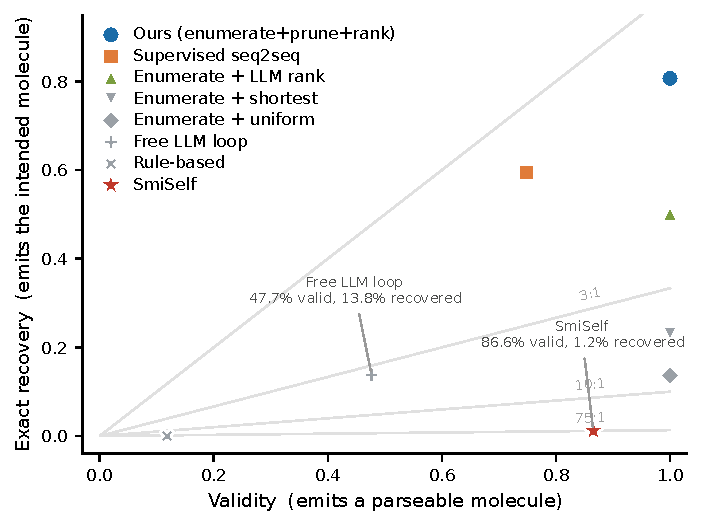
\includegraphics[width=0.78\linewidth]{fig_validity_recovery_plane.pdf}
\caption{Validity and recovery are close to independent. Grey lines are contours
of constant valid-outputs-per-correct-recovery. Two systems are annotated whose
relative ordering depends entirely on which axis is read.}
\label{fig:plane}
\end{figure}

\subsection{Experiment 2: can the candidate space contain the answer?}\label{sec:exp2}

Enumerating all single-token edits and keeping those RDKit accepts yields a
median of 50 candidate molecules per item (mean 75.9, 90th percentile 183). The
ground-truth molecule is in that set for \textbf{99.79\%} of test items. The
residual 0.21\% is concentrated in bracket corruptions, where a deleted closing
bracket sometimes cannot be repaired by a single token edit.

Two consequences follow. First, the task is essentially solvable within this
hypothesis space, so any shortfall is a \emph{ranking} failure, not a coverage
failure. Second, a system that picks uniformly at random from the candidate set
(with no learning whatsoever) achieves 12.7\% expected exact recovery,
which already exceeds every published system we evaluate. Figure~\ref{fig:space}
shows the distribution of candidate-set sizes and per-category coverage.

\begin{figure}[t]
\centering
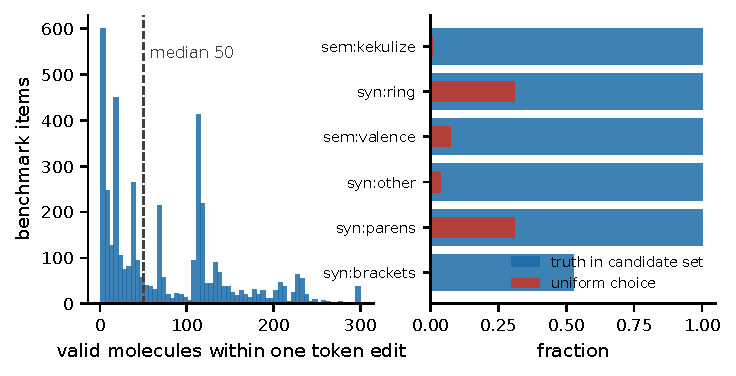
\includegraphics[width=0.92\linewidth]{fig_candidate_space.pdf}
\caption{Left: number of valid molecules within one token edit. Right: per error
category, the fraction of items whose candidate set contains the truth (blue)
and the expected accuracy of uniform selection (red).}
\label{fig:space}
\end{figure}

\subsection{Experiment 3: does symbolic pruning help?}\label{sec:exp3}

Using the RDKit diagnosis to discard edits inconsistent with the observed error
reduces the median candidate set from 45 to 28 on the development split while
leaving truth retention unchanged at 0.9978: the pruning is lossless. We
selected the constraint by sweeping candidate rules on the development split and
keeping the tightest lossless one; tightening kekulisation repairs to aromatic
atoms alone, for instance, would shrink the median set to 27 but drop retention
to 0.749, and was rejected.

\subsection{Experiment 4: does ranking matter?}\label{sec:exp4}

Holding the candidate set fixed and varying only the selection rule isolates the
contribution of the prior (Figure~\ref{fig:ladder}):

\begin{center}\small
\begin{tabular}{lr}
\toprule
Selection rule over the same candidate set & Exact recovery \\
\midrule
Uniform at random & 13.6\% \\
Shortest canonical SMILES & 23.1\% \\
General LLM likelihood (Qwen2.5-14B~\citep{qwen2025}, 14.7B params) & 50.2\% \\
Domain Transformer LM likelihood (3.2M params) & 75.4\% \\
Domain character-level LSTM likelihood (12.2M params) & \textbf{80.7\%} \\
\bottomrule
\end{tabular}
\end{center}

Each language-model rung uses the length normalisation that won on the
development split for that model, since the two families disagree about it: the
general LLM scores 47.7\% with summed and 39.3\% with mean log-likelihood, while
the character-level LSTM scores 80.3\% with mean and 77.9\% with summed. The
table below therefore reports each ranker at its own dev-selected setting; using
one rule for all of them would handicap whichever family it suited less.

The prior is worth 67 percentage points over uniform selection, and the gain
tracks domain-specificity rather than scale. Both domain language models beat the
general LLM by a wide margin while being thousands of times smaller: 75.4\% for a
3.2M-parameter Transformer and 80.7\% for the 12.2M-parameter character-level
LSTM, against 50.2\% for Qwen2.5-14B. Parameter count is not the operative
variable, since the smaller of the two domain models still exceeds a model four
thousand times its size. Their standing relative to each other is a separate
question: Section~\ref{sec:exp9} shows it depends on which generator produced the
data being repaired, so the gap between them here should not be read as an
architecture ranking. A model trained on SMILES places a sharper distribution
over molecular strings than a general-purpose model whose tokeniser fragments
them, and because both domain models see only a disjoint molecule split, their
advantage cannot be explained by recall of test molecules from web pretraining.

The gain is largest exactly where the problem is hardest. Kekulisation errors
are both the most frequent real failure (45.8\% of the benchmark) and the most
ambiguous (median 112 candidates even after pruning, 0.9\% uniform accuracy); the
domain prior lifts them to 67.5\%, a factor of 74. Ring closures go from 31.0\%
to 93.1\%, valence from 7.5\% to 87.4\% (Figure~\ref{fig:cat}).

\begin{figure}[t]
\centering
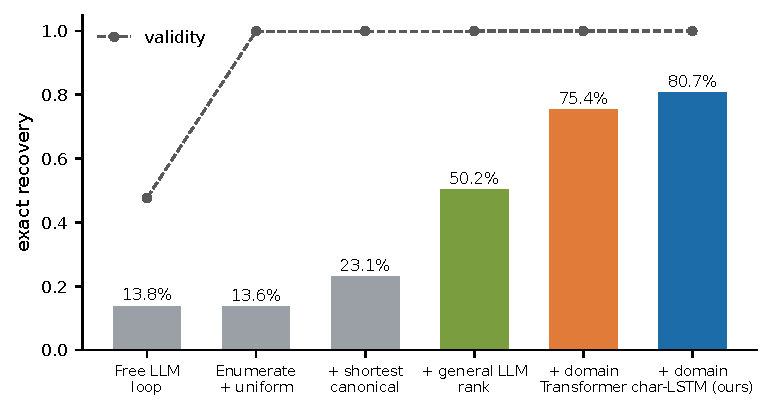
\includegraphics[width=0.8\linewidth]{fig_ranking_ladder.pdf}
\caption{Exact recovery (bars) and validity (dashed) as the free-generation loop
is replaced by enumeration and progressively better selection rules.}
\label{fig:ladder}
\end{figure}

\begin{figure}[t]
\centering
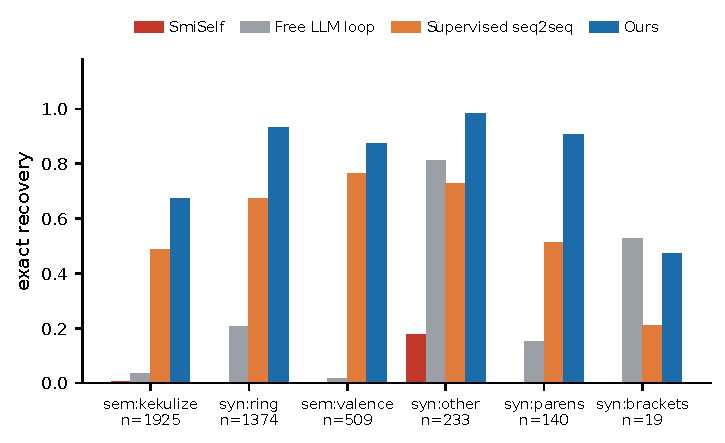
\includegraphics[width=0.92\linewidth]{fig_per_category.pdf}
\caption{Exact recovery by error category.}
\label{fig:cat}
\end{figure}

\begin{table}[t]
\centering\small
\caption{Representative recoveries. In every case the corruption is a single token, the toolkit localises the error, and the correct molecule is chosen from a candidate set of non-trivial size. Differences from the corrupted string are the only edit made.}
\label{tab:examples}
\begin{tabular}{@{}p{2.1cm}p{9.6cm}r@{}}
\toprule
Error type & Strings & $|C|$ \\
\midrule
\multirow{3}{*}{sem: kekulize} & \texttt{\footnotesize COc1cccc(CNC(=O)c2cc3ccc(-c4ccnc(N)c4)cc3[nH]2)1} \hfill\textit{\scriptsize in} \\
 & \texttt{\footnotesize COc1cccc(CNC(=O)c2cc3ccc(-c4ccnc(N)c4)cc3[nH]2)c1} \hfill\textit{\scriptsize out} \\
 & \texttt{\footnotesize COc1cccc(CNC(=O)c2cc3ccc(-c4ccnc(N)c4)cc3[nH]2)c1} \hfill\textit{\scriptsize truth} & 128 \\[2pt]
\multirow{3}{*}{syn: ring} & \texttt{\footnotesize CCN(CC)Cc1c(O)c(Cl)ccc(C)cc(=O)oc12} \hfill\textit{\scriptsize in} \\
 & \texttt{\footnotesize CCN(CC)Cc1c(O)c(Cl)cc2c(C)cc(=O)oc12} \hfill\textit{\scriptsize out} \\
 & \texttt{\footnotesize CCN(CC)Cc1c(O)c(Cl)cc2c(C)cc(=O)oc12} \hfill\textit{\scriptsize truth} & 12 \\[2pt]
\multirow{3}{*}{sem: valence} & \texttt{\footnotesize CC1=CC23OC2(CC(C)(C)C3=O)C(C)CFC1O} \hfill\textit{\scriptsize in} \\
 & \texttt{\footnotesize CC1=CC23OC2(CC(C)(C)C3=O)C(C)CCC1O} \hfill\textit{\scriptsize out} \\
 & \texttt{\footnotesize CC1=CC23OC2(CC(C)(C)C3=O)C(C)CCC1O} \hfill\textit{\scriptsize truth} & 17 \\[2pt]
\multirow{3}{*}{syn: parens} & \texttt{\footnotesize CSc1ccc(Oc2ccncc2CN(C)Ccc1Cl} \hfill\textit{\scriptsize in} \\
 & \texttt{\footnotesize CSc1ccc(Oc2ccncc2CN(C)C)cc1Cl} \hfill\textit{\scriptsize out} \\
 & \texttt{\footnotesize CSc1ccc(Oc2ccncc2CN(C)C)cc1Cl} \hfill\textit{\scriptsize truth} & 11 \\[2pt]
\multirow{3}{*}{syn: other} & \texttt{\footnotesize Cc1cc(C)cc(NC(==S)N2CCC(C(=O)c3ccc(F)cc3)CC2)c1} \hfill\textit{\scriptsize in} \\
 & \texttt{\footnotesize Cc1cc(C)cc(NC(=S)N2CCC(C(=O)c3ccc(F)cc3)CC2)c1} \hfill\textit{\scriptsize out} \\
 & \texttt{\footnotesize Cc1cc(C)cc(NC(=S)N2CCC(C(=O)c3ccc(F)cc3)CC2)c1} \hfill\textit{\scriptsize truth} & 36 \\
\bottomrule
\end{tabular}
\end{table}


\paragraph{Free generation is the wrong mechanism.}
Our own earlier system is instructive as a negative result. Adding symbolic
feedback and iteration to an LLM repair loop raises validity monotonically
(23.4\% $\rightarrow$ 27.0\% $\rightarrow$ 37.4\% $\rightarrow$ 47.7\%) but
recovery saturates near 13.8\%, and the iterative variants actually
\emph{reduce} Tanimoto (0.737 $\rightarrow$ 0.660) and scaffold match (48.5\%
$\rightarrow$ 34.9\%). The loop buys validity by drifting away from the intended
molecule. Constrained selection over the same problem reaches 100\% validity and
80.7\% recovery simultaneously, which is why we conclude that invalid-SMILES
recovery is better formulated as constrained candidate selection than as
unconstrained sequence generation.

Across three seeds the free loop varies by 0.15 percentage points
(13.79/13.64/13.79\%), far below the gaps between conditions.

\subsection{Experiment 5: does it beat supervised correction?}\label{sec:exp5}

The obvious alternative is to train a dedicated corrector. We took the
transformer architecture of~\citet{schoenmaker2023uncorrupt} and retrained it from
scratch on 245{,}000 corrupted/correct pairs generated \emph{from our own
corruption distribution}, so that it suffers no domain shift, using molecules
disjoint from the benchmark. This baseline is given every advantage the setting
allows.

It reaches 74.8\% validity and 59.4\% exact recovery, far better than the
validity-oriented systems of Section~\ref{sec:exp1} (SmiSelf at 1.2\%,
rule-based repair at 0.0\%), confirming that in-distribution supervision on the
right objective matters a great deal, and still 21 points below \ours{} (paired
McNemar $+1210/-318$, $p_{\text{Bonf}} = 1.1\times10^{-121}$). The supervised
corrector also inherits the generative failure mode: one output in four does not
parse at all, whereas enumeration makes invalidity impossible.

\ours{} matches that result with \emph{no repair supervision}, requiring only a
chemistry toolkit, which practitioners already have, and a generative chemical
language model, which in the intended deployment is the very model whose outputs
are being repaired.

\subsection{Experiment 6: does it transfer to real generator failures?}\label{sec:exp6}

Our benchmark corrupts molecules deliberately, which invites the objection that
real generative models might fail in ways the operators do not capture. To test
that, we apply the pipeline to 4{,}009 genuinely invalid SMILES sampled from our
character-level generator at $T=1.0$, and to a second benchmark built by
corrupting the generator's \emph{own} valid outputs.

\paragraph{The one-edit hypothesis space holds on real failures.}
Enumerating single-token repairs for the real failures yields a non-empty
candidate set for \textbf{91.5\%} of them (median 72 candidates). The design
assumption thus holds of real generator output and is not an artefact of how we
built the benchmark. The remaining 8.5\% carry more than one simultaneous
error and are outside the current enumerator; we return them unchanged rather
than guessing, which is the correct behaviour for a system that is asked to
preserve identity.

\paragraph{Identity preservation without ground truth.}
Exact recovery cannot be measured on real failures, since nobody knows which
molecule the model intended, and that is precisely why the controlled benchmark
exists. What can be measured is how much of the string a repair destroys. A
method that rewrites most of the molecule cannot be preserving what the
generator was reaching for, whatever its validity rate.

\begin{center}\small
\begin{tabular}{lrrr}
\toprule
On 4{,}009 real generator failures & Yield & \multicolumn{2}{c}{Repair size (tokens)} \\
\cmidrule(l){3-4}
 & (valid output) & median & mean \\
\midrule
\ours{} (ours)              & 91.5\% & \textbf{1} & \textbf{1.00} \\
SmiSelf~\citep{smiself2025} & 90.9\% & 21 & 21.47 \\
\bottomrule
\end{tabular}
\end{center}

\noindent
Repair size is the token edit distance from the broken string to the string the
method emitted. Every \ours{} repair is a single token by construction.
(Measured instead against the \emph{canonicalised} output, our median rises to 2
and the mean to 9.8, but that reflects RDKit re-serialising the string rather
than any further change to the molecule; we report the applied edit, which is
the quantity of interest.)

SmiSelf converts a comparable fraction of real failures into valid molecules, but
at a median token edit distance of 21: it re-encodes the string through SELFIES
and emits a largely different molecule. On the controlled benchmark that
difference is worth 1.2\% against 80.7\% exact recovery. Here the truth is
unknown, so the 21-fold gap in intervention size is the only trace of the same
effect we can observe.

\paragraph{Recovery on the generator's own distribution.}
To obtain ground truth on the distribution a real model actually produces, we
corrupted 2{,}000 of the generator's own valid outputs with the same operators.
Because these molecules came from the generator, ground truth is available and
exact recovery is measurable. The candidate set contains the truth for 99.7\% of
items (median 47 candidates) and uniform selection scores 12.5\%, both close to
the main benchmark. \ours{} recovers 78.9\% exactly at 99.9\% validity, against
80.7\% on the GuacaMol-derived benchmark.

The method transfers to the distribution a real model produces, losing under two
points. Note also that the ranker here is the very model that generated the
molecules, so the prior is matched to the data: the deployment setting, but
equally the configuration in which one would most expect an inflated result.
Performance is slightly \emph{lower} than on molecules the ranker has never seen,
which argues that the chemical prior, rather than familiarity with these
particular molecules, is doing the work.

\subsection{Experiment 7: where does the one-edit assumption break?}\label{sec:exp7}

Enumerating single-token edits is the assumption the method rests on, so we
measure what it costs. Using the same held-out pool but excluding all 6{,}000
molecules of the main benchmark, we built matched benchmarks of 600 items at
$k=1$, $2$ and $3$ simultaneous edits (realised mean token distance 1.10, 2.01,
3.29).

\begin{center}\small
\begin{tabular}{crrr}
\toprule
$k$ (simultaneous edits) & one-edit coverage & median candidates & empty sets \\
\midrule
1 & \textbf{99.67\%} & 45 & 0/600 \\
2 & 0.50\% & 0 & 324/600 \\
3 & 0.00\% & 0 & 536/600 \\
\bottomrule
\end{tabular}
\end{center}

\noindent
The enumerator does not degrade gracefully. It is near-complete at $k=1$ and of
almost no use at $k=2$, which fixes the method's scope boundary and makes the
measurement in Section~\ref{sec:exp6} load-bearing: 91.5\% of \emph{real}
generator failures fall on the useful side of it. On the $k=1$ benchmark, whose molecules
are disjoint from the main benchmark entirely, \ours{} recovers \textbf{80.0\%}
exactly at 100\% validity, replicating the 80.7\% headline on fresh molecules.

\paragraph{Buying a second edit, and what it costs.}
A complete two-edit enumeration is quadratic and infeasible. We therefore run a
bounded search: level one enumerates one-edit neighbours; the invalid ones are
ranked by a purely syntactic imbalance score (unclosed branches, odd
ring-closure digits, bracket mismatch, none of which uses ground truth), and the best
\emph{beam} of them are expanded by a second edit under a per-item wall-clock
budget.

\begin{center}\small
\begin{tabular}{lrrrr}
\toprule
Configuration & $n$ & $k{=}2$ coverage & parses/item & s/item \\
\midrule
one-edit only            & 600 & 0.5\%           & $\sim$5k    & $\sim$0.02 \\
beam 60, 4\,s budget     & 40  & 5.0\%           & 28{,}063    & 4.42 \\
beam 150, 15\,s budget   & 20  & 30.0\%          & 117{,}819   & 15.32 \\
beam 400, 60\,s budget   & 12  & \textbf{58.3\%} & 437{,}774   & 60.32 \\
\bottomrule
\end{tabular}
\end{center}

\noindent
Coverage rises monotonically and the budget binds at every setting (truncation
on 100\%, 100\% and 92\% of items respectively), so each figure is a lower bound
for that compute level. What limits the search is compute rather than the ranking
heuristic. The second edit is reachable, at roughly three orders of magnitude
more work than the first. We report this as a cost curve and do not claim to
solve the multi-edit case.

\subsection{Experiment 8: an external benchmark, built by someone else}\label{sec:exp8}

Both the corruption operators and the source molecules are ours, which leaves
open whether the method is tuned to its own corruption process. We therefore built an independent
benchmark using the corruption code released with UnCorrupt
SMILES~\citep{schoenmaker2023uncorrupt}, at one error per molecule, applied to
their molecule source (PAPYRUS, a bioactivity corpus). The operators, the
fragment library and the molecules are all theirs; our ranker has never seen a
PAPYRUS molecule, so the benchmark doubles as an out-of-distribution test of the
chemical prior ($n = 1{,}200$). This reconstructs the condition
\citet{schoenmaker2023uncorrupt} evaluate themselves, so their published figure is
the natural reference point: 70.5\% reconstruction at one error per input, and
78\% for their translator overall. The comparison is indicative rather than
like-for-like, since their model is trained on this corruption distribution and
ours is not, their evaluation set is their own validation split, and the operator
mix differs from the one we sample. It is nonetheless the closest direct point of
contact between the two systems, and we report it rather than leave it to be
inferred.

Their notion of ``one error'' is not one token: only 28.0\% of items lie a single
token from the intended molecule, the median is 5, the 90th percentile is 26, and
11.1\% graft an entire fragment onto the molecule (in which case the intended
target is the grafted molecule, and we score against it exactly as their own
pipeline does). Spanning both sides of our scope boundary makes it a stress test
rather than a like-for-like comparison.

\begin{center}\small
\begin{tabular}{lr}
\toprule
\ours{} on the external benchmark ($n=1{,}200$) & \\
\midrule
truth reachable within one edit          & 69.1\% \\
items answered (non-empty candidate set) & 84.5\% \\
\quad validity $\mid$ answered           & \textbf{100.00\%} \\
\quad recovery $\mid$ answered           & 71.5\% \\
items abstained (empty candidate set)    & 15.5\% \\
\midrule
overall validity                         & 84.5\% \\
overall exact recovery                   & \textbf{60.4\%} \\
Tanimoto $\mid$ valid                    & 0.888 \\
scaffold match $\mid$ valid              & 77.4\% \\
\midrule
recovery $\mid$ truth reachable          & \textbf{87.5\%} \\
recovery $\mid$ truth not reachable      & \textbf{0.00\%} \\
\bottomrule
\end{tabular}
\end{center}

\paragraph{How much of this benchmark is reachable at all.}
String edit distance is the wrong axis here. Their \texttt{permutation} operator
reorders tokens and their graft operator appends a whole fragment, both of which
inflate string distance while leaving the required repair small, and
canonicalisation inflates it further. We report \emph{reachability} instead. The truth is reachable within one edit for 69.1\% of items. Of the 371
that are not, a bounded two-edit search (beam 150, 15\,s per item; probe of 120)
reaches a further 5.0\%, about 1.5 points, with the budget binding on every
item, again a lower bound. Roughly 29\% of this external benchmark lies beyond
edit-bounded enumeration altogether. That is the limit of the approach: it is a
precise repair mechanism, not a general molecule reconstructor.

\noindent
Recovery conditioned on the truth being reachable is 87.5\%, marginally
\emph{higher} than the corresponding figure on our own benchmark (80.7\% of
99.8\%, i.e.\ 80.9\%), so the chemical prior transfers to an unseen molecule
corpus with no loss we can detect. The two figures are close enough that we
draw no conclusion from the direction of the difference. Two of the remaining entries are checks rather than
results. Recovery conditioned on the truth \emph{not} being reachable is exactly
zero: the method cannot return a molecule it never enumerated. Validity
conditioned on answering is exactly 100\%, on data the system was never designed
against. The 15.5\% it declines are the multi-edit corruptions of
Experiment~\ref{sec:exp7}, and declining them is the correct behaviour for a
system whose purpose is to preserve identity.

\subsection{Experiment 9: does the prior have to match the generator?}\label{sec:exp9}

Our ranker is the generative model whose output is being repaired, which is the
intended deployment but raises the question of how much of the performance comes
from that match. To separate the two, we trained a second generator of a
different family (a 3.2M-parameter decoder-only SMILES Transformer, trained on
the same corpus and reusing the character vocabulary of the LSTM verbatim, so
the comparison is architectural rather than a tokenisation artefact), and built a
corruption benchmark from each generator's own valid samples (2{,}000 items
each, identical operators and seed). The two generators differ substantially in
how often they fail: 93.3\% of the LSTM's samples parse, against 83.6\% of the
Transformer's. Their failures are nonetheless equally reachable (candidate-set
coverage 99.7\% and 99.8\%, median 47 and 44 candidates), so differences below
are attributable to the ranker rather than to one benchmark being easier.

\begin{center}\small
\begin{tabular}{lcc}
\toprule
& \multicolumn{2}{c}{Ranker} \\
\cmidrule(l){2-3}
Benchmark (corruptions of\ldots) & char-LSTM (12.2M) & Transformer (3.2M) \\
\midrule
LSTM's own molecules       & \textbf{78.9\%} & 73.1\% \\
Transformer's own molecules & 64.9\% & \textbf{73.8\%} \\
\midrule
GuacaMol test (neither generator's) & \textbf{80.7\%} & 75.4\% \\
\bottomrule
\end{tabular}
\end{center}

\noindent
The diagonal dominates. Each ranker recovers best on the benchmark built from its
own generator's molecules, the LSTM ahead by 5.8 points on LSTM-derived
corruptions and the Transformer ahead by 8.8 points on Transformer-derived ones;
averaged over the two, a matched prior is worth 7.3 points (76.3\% against
69.0\%).

What the table shows is an interaction rather than an ordering. It supports the
deployment we assume, namely repairing a generator's output with that generator, whose
prior is calibrated to the region of chemical space where it is producing broken
strings. It also accounts for the five-point gap between the two domain models in
Section~\ref{sec:exp4}, which is not evidence that recurrent architectures rank
better: that benchmark simply happens not to be Transformer-derived, and on
Transformer-derived data the ordering reverses. The cost of a mismatch is
bounded, since even the worse off-diagonal cell (64.9\%) remains above the
general-LLM ranker (50.2\%) and far above the validity-oriented corrector
evaluated here (1.2\%), so a mismatched domain prior degrades recovery without
destroying it.

Validity is 99.9\% or above in all four cells, as it must be, since enumeration
guarantees it regardless of which model does the ranking.

\subsection{Statistical significance}

All differences in Table~\ref{tab:main} are significant under exact paired
McNemar tests with Bonferroni correction ($m=6$):

\begin{center}\small
\begin{tabular}{lrr}
\toprule
Comparison (exact recovery) & wins/losses & $p_{\text{Bonf}}$ \\
\midrule
\ours{} vs.\ SmiSelf                & $+3344/-5$    & $<10^{-300}$ \\
\ours{} vs.\ shortest canonical     & $+2453/-34$   & $<10^{-300}$ \\
\ours{} vs.\ general-LLM ranking    & $+1427/-146$  & $1.7\times10^{-263}$ \\
\ours{} vs.\ supervised seq2seq     & $+1210/-318$  & $1.1\times10^{-121}$ \\
Supervised seq2seq vs.\ SmiSelf     & $+2460/-13$   & $<10^{-300}$ \\
Supervised seq2seq vs.\ LLM ranking & $+996/-607$   & $1.2\times10^{-21}$ \\
\bottomrule
\end{tabular}
\end{center}

\subsection{Contamination check}\label{sec:contam}

Exactly one test molecule occurs in the corpus used to train the generator and
ranker. Removing it and recomputing every headline number changes \ours{} by
$-0.005$ percentage points (80.67\% $\rightarrow$ 80.66\%); across all systems
the largest change is 0.02 points. Training-set contamination does not explain
these results.

\subsection{Calibrated abstention}\label{sec:abstain}

Because recovery is not perfect, a deployable system should know when it is
unsure. The gap between the top-ranked and second-ranked candidate
log-likelihood is a confidence signal that never consults ground truth. Sorting
test items by it yields the risk--coverage curve in Figure~\ref{fig:risk}. The
signal is defined for the 3{,}881 items (92.4\%) whose pruned candidate set holds
more than one molecule; the remaining 319 admit a single candidate and involve no
ranking decision. Among those 3{,}881, answering the most confident 50\% gives
96.4\% precision, the most confident 30\% gives 99.2\%, and the most confident
20\% gives 99.7\%. The 50\% operating point is 1{,}940 molecules, or 46\% of the
full test split.

\begin{figure}[t]
\centering
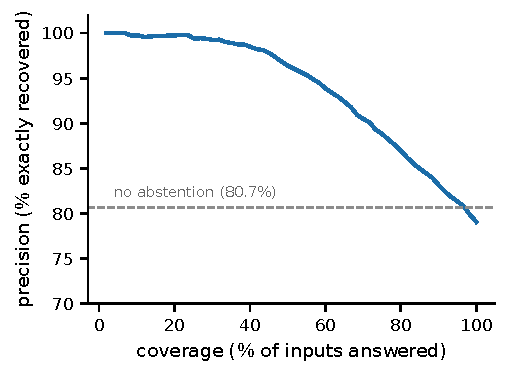
\includegraphics[width=0.6\linewidth]{fig_risk_coverage.pdf}
\caption{Risk--coverage curve for \ours{}, over the 3{,}881 test items for which
the ranking margin is defined. Answering the most confident half of them (46\%
of the full test split) gives 96.4\% precision.}
\label{fig:risk}
\end{figure}

\section{Discussion}

\paragraph{What the field should report.}
We do not argue that validity is meaningless: a system that emits unparseable
strings is useless. We argue that validity is insufficient, and that reporting
it alone permits a system to look excellent while recovering almost nothing. The
$\mathrm{V/R}$ ratio is a cheap diagnostic: any corrector whose ratio is far
from 1 is mostly manufacturing molecules rather than recovering them. Recovery
metrics require ground truth, which is exactly what a benchmark like ours
supplies.

\paragraph{Where the difficulty actually lives.}
The decomposition is clean. Symbolic enumeration makes recovery \emph{possible}
: it delivers a sound candidate set containing the answer 99.79\% of the time.
The chemical prior makes recovery \emph{accurate}, converting 12.7\% into
80.7\%. Neither half suffices alone: enumeration without a prior is barely
better than published methods, and a prior without enumeration (the free LLM
loop) sacrifices validity and drifts off the intended molecule.

\paragraph{Limitations.}
Our benchmark applies single-token corruptions. This matches the modal real
failure, and Section~\ref{sec:exp6} shows that 91.5\% of real generator failures
admit a one-edit repair, but the remaining 8.5\% carry multiple simultaneous
errors and are outside the current enumerator. Section~\ref{sec:exp7}
quantifies that boundary rather than assuming it: coverage falls from 99.7\% at
one edit to 0.5\% at two and 0.0\% at three, and a bounded two-edit search
recovers much of the $k{=}2$ case (58.3\% coverage) only at roughly three orders
of magnitude more compute. Bracket corruptions expose a further ceiling of the
one-edit hypothesis space (52.6\% coverage on that category, $n=19$). Finally,
our ranker is the generator itself, which is the intended deployment;
Section~\ref{sec:exp6} indicates this does not inflate results and
Section~\ref{sec:exp8} shows the prior transfers undegraded to a molecule corpus
it never saw, but the cost of a deliberately adversarial mismatch remains
uncharacterised.

\section{Conclusion}

Validity has served as the default metric for SMILES correction. We find that
it can substantially mis-rank systems: a published corrector attains 86.6\% validity
while recovering the intended molecule for 1.2\% of inputs, and is ordered ahead
of a system that recovers twelve times as many molecules. Once recovery is
measured directly, the problem changes shape. It is better posed as constrained
selection than as generation: enumerate the repairs a chemistry toolkit will
accept, prune them with the toolkit's own diagnosis, and let a chemical language
model choose. That system recovers the intended molecule for 80.7\% of held-out
corrupted strings at 100\% validity, beats a supervised corrector trained on
245k in-distribution repair pairs, and supports abstention at 96.4\% precision
over 46\% of its inputs.


\section*{Declarations}

\paragraph{Availability of data and materials.}
The recovery benchmark (6{,}000 corrupted SMILES with ground truth, split into
development and test), the multi-edit and external benchmarks, all per-item
system outputs, and the code reproducing every table and figure are available at
\url{https://github.com/Sridharasyamch/validity-is-not-recovery}. The trained
generators and the supervised-corrector baseline are published as release assets
in the same repository. The enumerated candidate sets and the 245{,}000-pair
supervised-training corpus are omitted for size and regenerate deterministically
from the released code. Source molecules are from the public GuacaMol/ChEMBL
corpus. The code is released under the MIT licence.
Baseline weights for the supervised corrector were trained by us; SmiSelf was run
from its authors' released implementation.

\paragraph{Ethics approval and consent to participate.}
Not applicable. This work involves no human participants, human data, or animals.

\paragraph{Consent for publication.}
Not applicable.

\paragraph{Competing interests.}
The authors declare no competing interests.

\paragraph{Funding.}
Not applicable.

\paragraph{Authors' contributions.}
All authors contributed equally to this work. They jointly conceived the study,
designed the benchmark and evaluation protocol, developed and implemented the
method, analysed the results, and wrote and approved the manuscript.

\paragraph{Acknowledgements.}
Not applicable.

\bibliographystyle{unsrtnat}
\bibliography{references}

\end{document}
